\chapter{Аналитический раздел}

В данном разделе описывается и визуализируется набор данных, формализуется задача, проводится анализ существующих моделей регрессии осуществляется выбор наиболее подходящей для решения поставленной задачи, а также выбирается функционал качества модели.

\section{Описание и анализ набора данных}
Набор данных, на основе которого разрабатывается система предсказания выпускного балла по образу жизни студентов, состоит из следующих признаков:
\begin{enumerate}
    \item school -- название школы (бинарный: 'GP' -- Gabriel Pereira, 'MS' - Mousinho da Silveira);
    \item sex -- пол (бинарный: 'F' -- женский; 'M' -- мужской);
    \item age -- возраст (числовой: от 15 до 22);
    \item addres -- тип места жительства (бинарный: 'U' -- город, 'R' - деревня);
    \item famsize -- размер семьи (бинарный: 'LE3' -- меньше 3, 'GT3' -- больше 3);
    \item pstatus -- статус родителей (бинарный: 'T' -- живут вместе, 'A' -- отдельно);
    \item medu -- образование матери (числовой: 0 -- нет образования, 1 -- начальное, 2 -- базовое среднее, 3 -- полное среднее, 4 -- высшее);
    \item fedu -- образование отца (числовой: 0 -- нет образования, 1 -- начальное, 2 -- базовое среднее, 3 -- полное среднее, 4 -- высшее);
    \item mjob -- работа матери (номинальный: 'teacher' -- учитель, 'health' -- связан со здровоохранением, 'services' -- гражданские сервисы, 'at\_home' -- не трудоустроен, 'other' -- другое);
    \item fjob -- работа отца (номинальный: 'teacher' -- учитель, 'health' -- связан со здровоохранением, 'services' -- гражданские сервисы, 'at\_home' -- не трудоустроен, 'other' -- другое);
    \item reason -- причина выбор школы (номинальный: 'home' -- близко к дому, 'reputation' -- репутация школы, 'course' -- предпочтительная образовательная программа, 'other' -- другое);
    \item guardian -- опекун (номинальный:  'mother' -- мать, 'father' -- папа, 'other' -- другое);
    \item traveltime -- время пути в школу (числовой: 1 -- меньше 15 минут, 2 -- от 15 минут до 30 минут, 3 -- от 30 минут до 45 минут, 4 -- больше часа);
    \item studytime -- время на самостоятельную подготовку в неделю (числовой: 1 -- меньше 2 часов, 2 -- от 2 до 5 часов, 3 -- от 5 до 10 часов, 4 -- больше 10 часов);
    \item failures -- количество проваленных контрольных (числовое: если n в диапазоне 1-3, то n, иначе 4);
    \item schoolsup -- дополниьельные занятия (бинарный: 'yes' -- да, 'no' -- нет);
    \item famsup -- помощь семьи в учёбе (бинарный: 'yes' -- да, 'no' -- нет);
    \item paid -- дополнительные оплачиваемые занятия (бинарный: 'yes' -- да, 'no' -- нет);
    \item activities -- наличие хобби (бинарный: 'yes' -- да, 'no' -- нет);
    \item nursery -- посещал ли детский сад (бинарный: 'yes' -- да, 'no' -- нет);
    \item higher -- хоачет получить высшее образование (бинарный: 'yes' -- да, 'no' -- нет);
    \item internet -- есть доступ в интернет дома (бинарный: 'yes' -- да, 'no' -- нет);
    \item romantic -- состоит в романтических отношениях (бинарный: 'yes' -- да, 'no' -- нет);
    \item famrel -- качество отношений в семье (числовое: от 1 -- плохо до 5 -- хорошо);
    \item freettime -- свободное время после занятий (числовое: от 1 -- мало до 5 -- много);
    \item goout -- ходит на прогулки с друзьями (числовое: от 1 -- редко до 5 -- часто);
    \item dalc -- употребляет алкоголь в рабочие дни (числовое: от 1 -- редко до 5 -- часто);
    \item walc -- употребляет алкоголь в выходные дни (числовое: от 1 -- редко до 5 -- часто);
    \item health -- здоровье (числовое: от 1 -- слабое до 5 -- хорошее);
    \item absences -- прогулы (числовое: от 0 до 93);
    \item G1 -- оценка за 1 семестр (числовое: от 0 до 20);
    \item G2 -- оценка за 2 семестр (числовое: от 0 до 20);
    \item G3 -- итоговая оценка (числовое: от 0 до 20).
\end{enumerate}

Выпускной балл, который необходимо предсказать, ялвяется признаком с названием G3. Распределение этого признака показано на рисунке \ref{fig:g3-hist}.

\begin{figure}[h!]
	\centering
	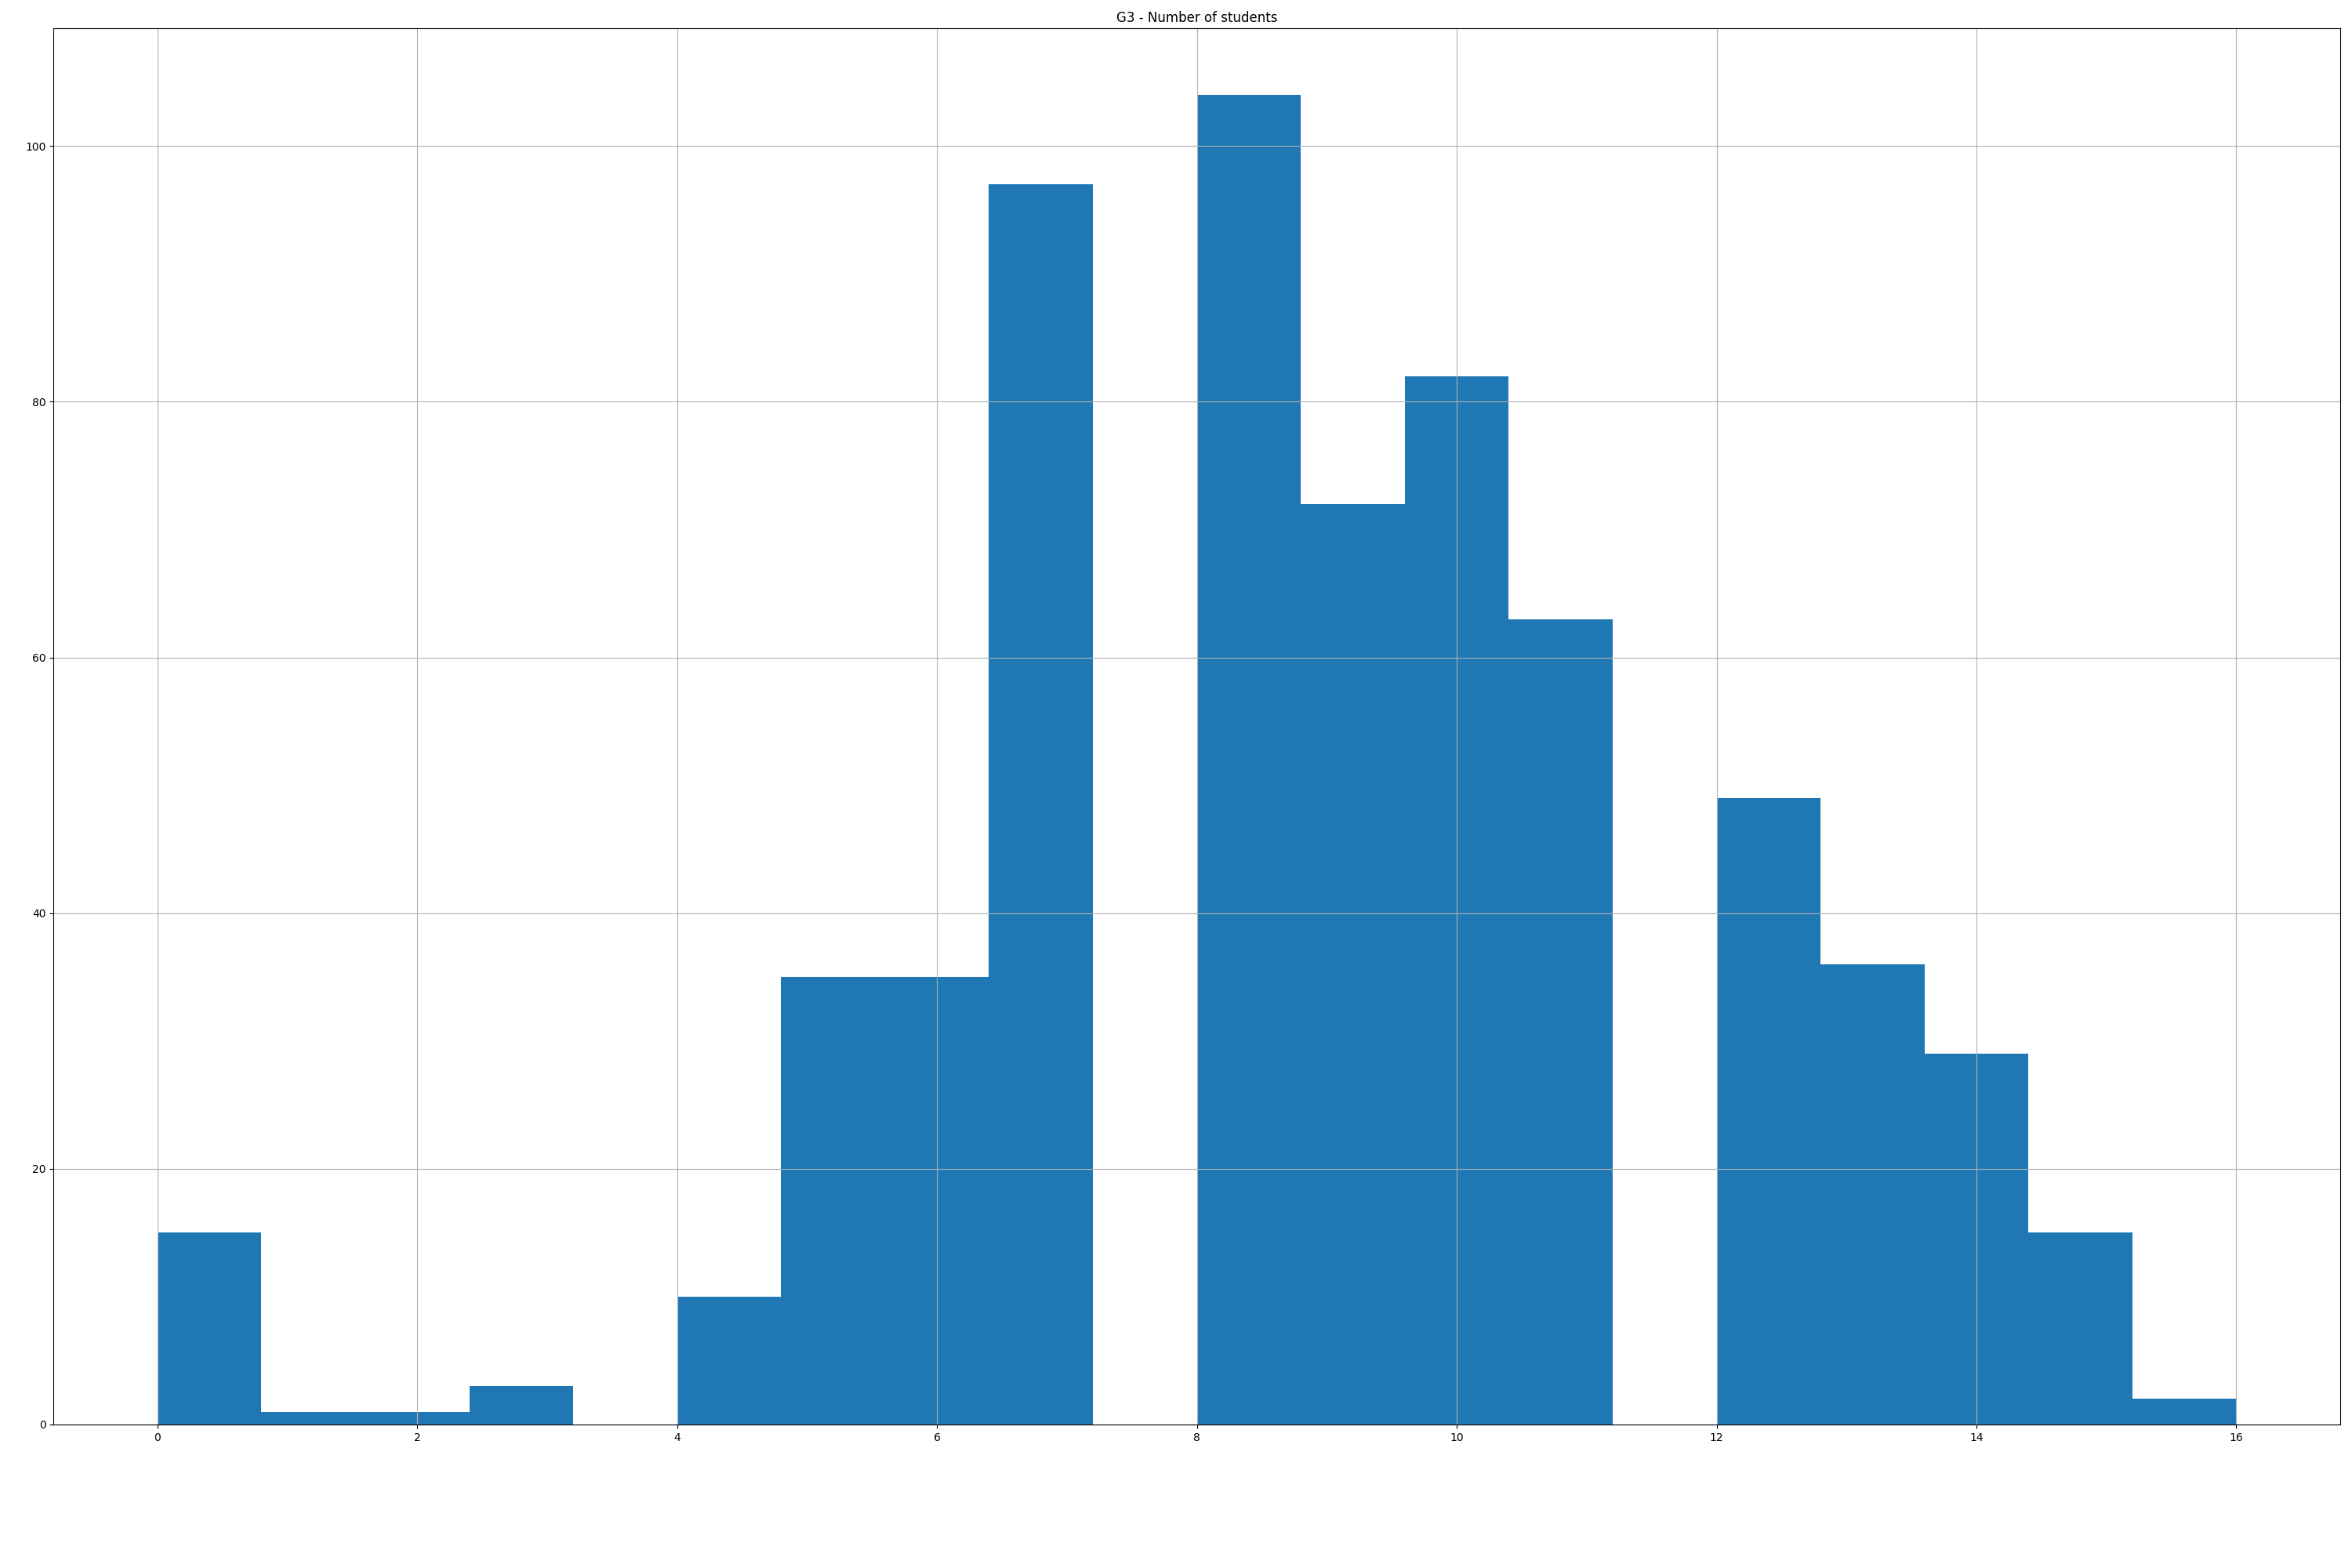
\includegraphics[scale = 0.13]{img/G3_hist.png}
	\caption{Распределение G3}
	\label{fig:g3-hist}
\end{figure}


Из описания признаков предлагается исключить признак school, поскольку он не является показательными с точки зрения образа жизни студентов. Кроме того, все номинальные и бинарные признаки необходимо предобработать, превратив их в числовые.

На рисунке \ref{fig:corr-matrix} приведена матрица корреляции признаков.
\begin{figure}[h!]
	\centering
	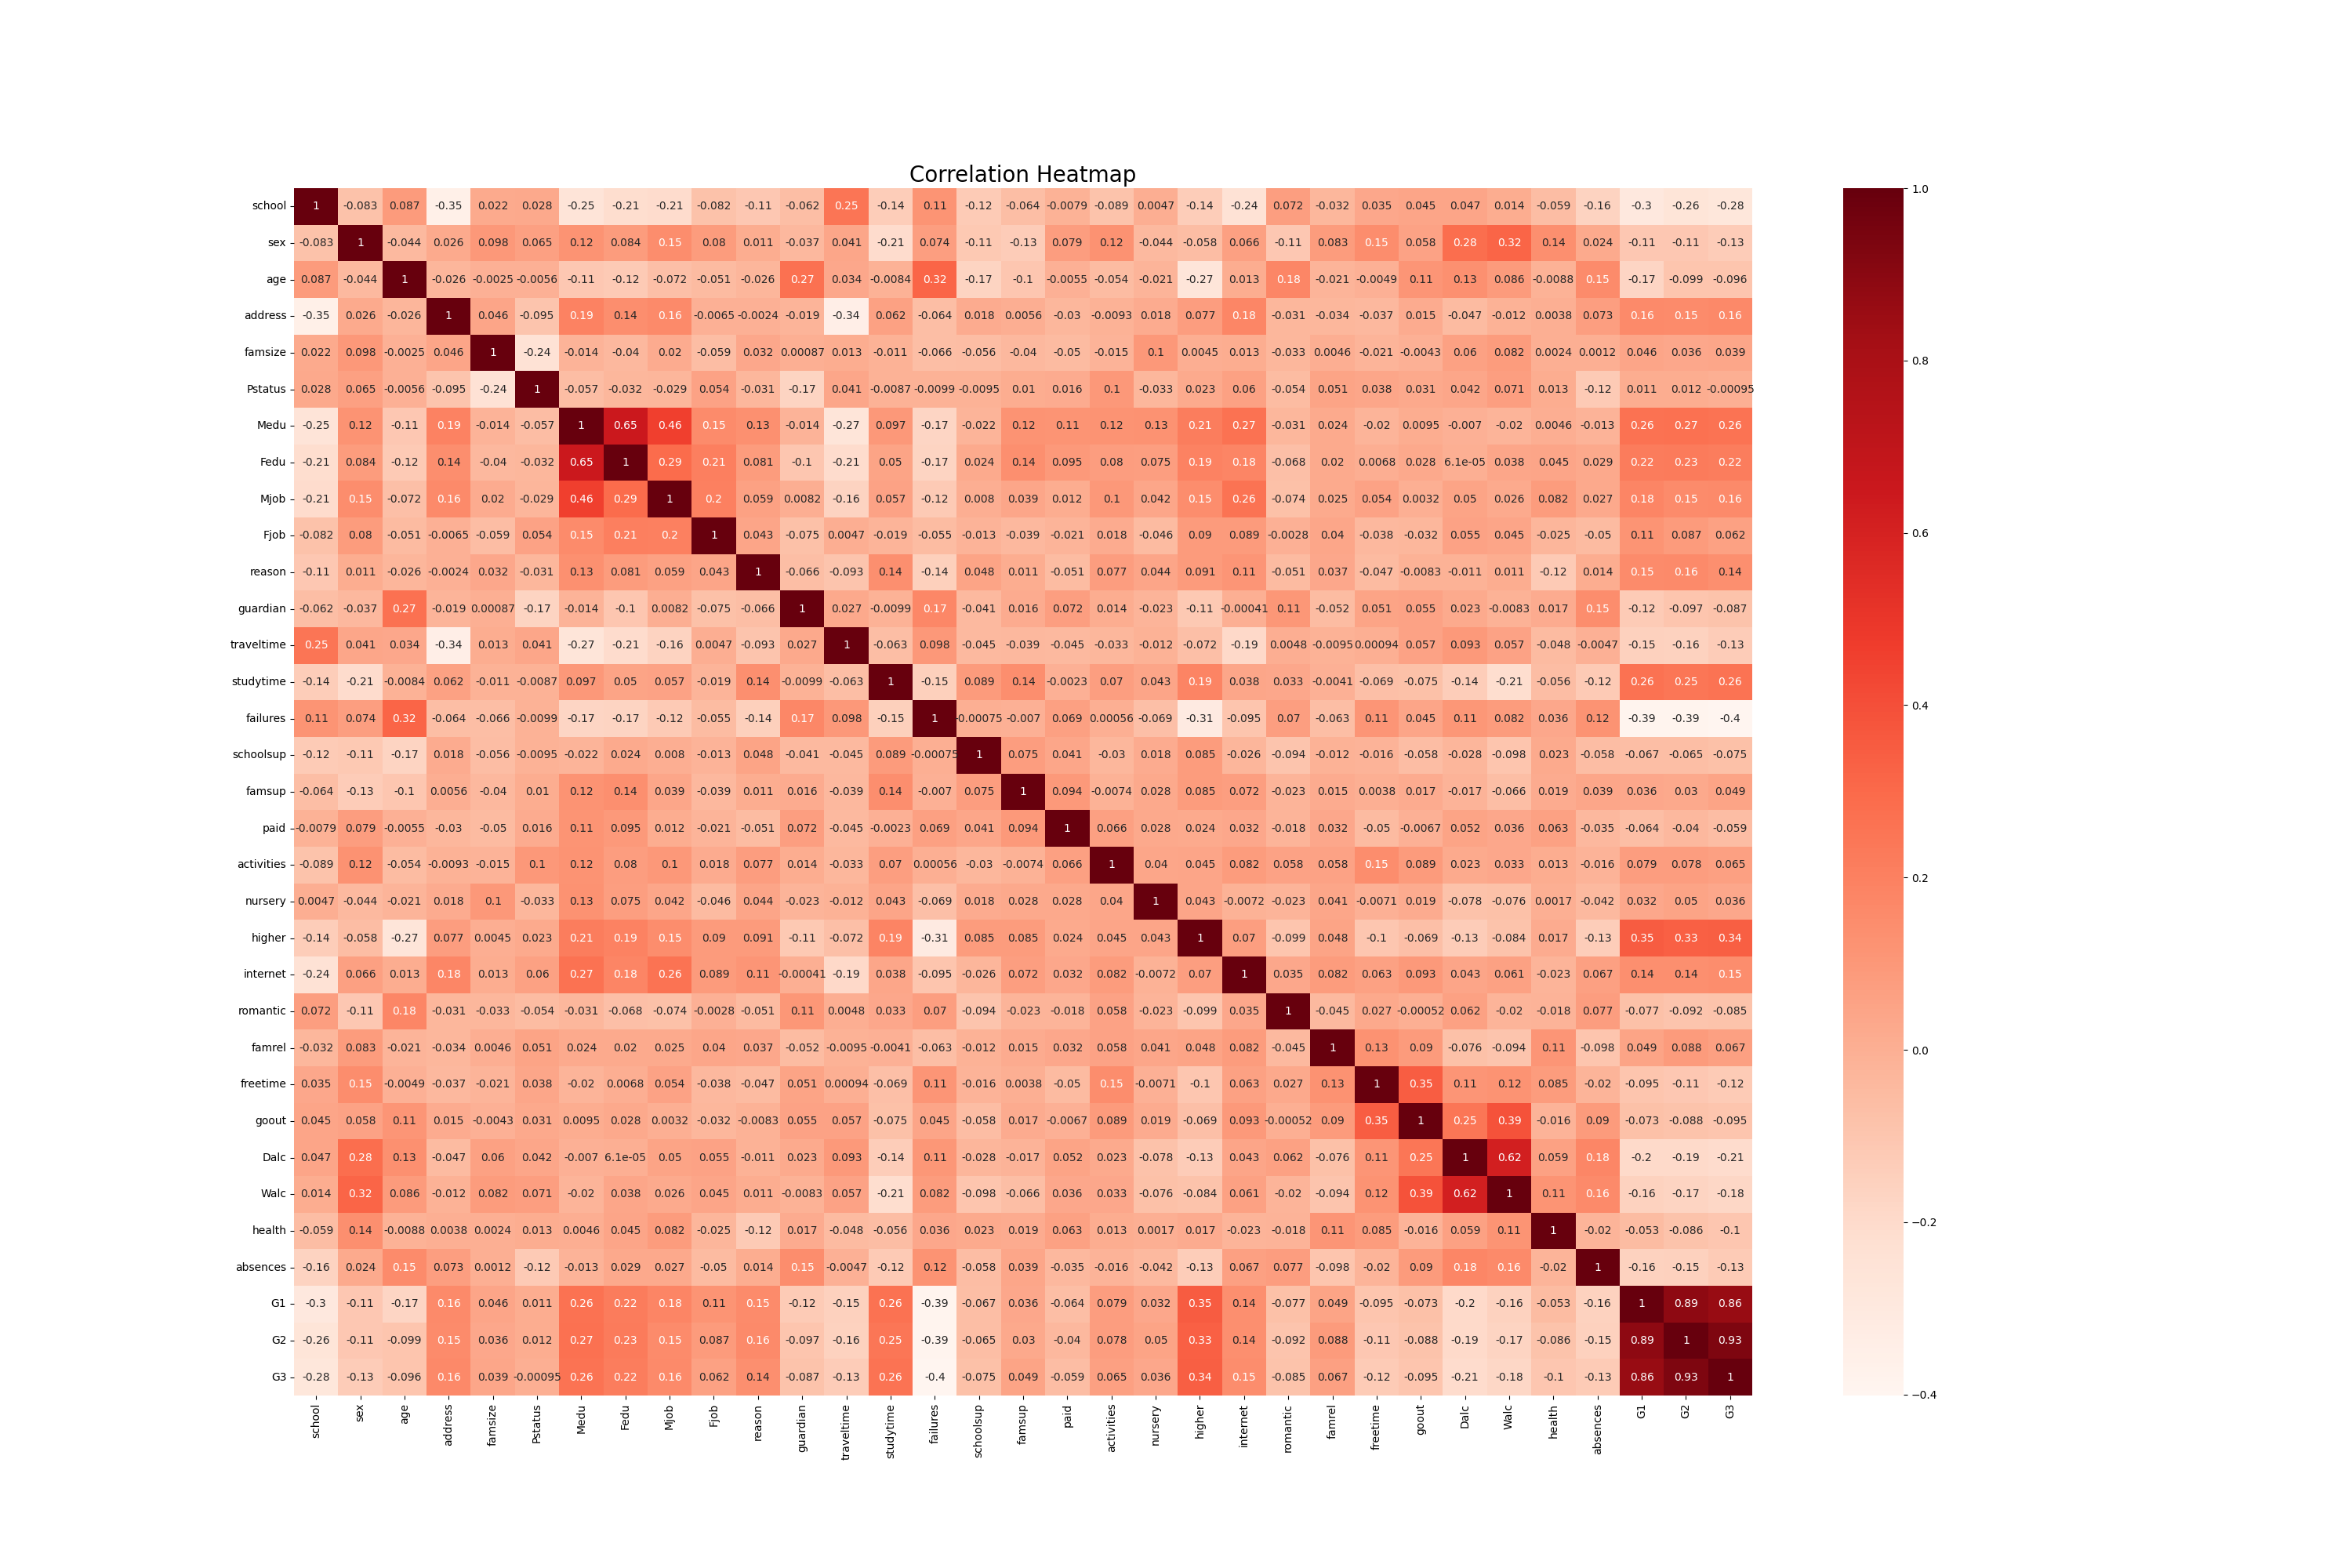
\includegraphics[width = \linewidth]{img/correlation.png}
	\caption{матрица корреляции признаков}
	\label{fig:corr-matrix}
\end{figure}

Видно, что признаки G1 и G2 сильно коррелируют с G3, что логично, ведь G1 и G2 являются оценками за экзамены предыдущих семестров. Это значит, что любая модель будет принимать во внимание только эти признаки, что нежелательно, поэтому исключим их из признаков перед обучением модели.


\section{Формализация задачи}

Требуется разработать систему предсказания выпускного балла студентов (признак G3) на основе их образа жизни (остальные признаки, которые не были исключены в анализе набора данных X). Математически это может быть описано следующим образом.

Дано обучающее множество:
\begin{equation}
    {(x^{1}, y^{1}), (x^{2}, y^{2}), …, (x^{m}, y^{m})}
\end{equation}
    
где:
\begin{itemize}
    \item $x^{i} = (x_1^{i}, x_2^{i}, …, x_n^{i})$ -- вектор входных признаков для i-го студента;
    \item $y^{i}$ -- соответствующее выходное значение (значение G3).
\end{itemize}

Цель -- найти функцию $f(x)$ (модель), которая будет предсказывать выходное значение $y$ по входным признакам $x$. Обычно эта функция задается параметрическим семейством моделей. Для настройки параметров модели используется метод оптимизации, например, метод наименьших квадратов или градиентный спуск. Цель состоит в том, чтобы минимизировать функцию потерь, которая измеряет разницу между предсказанными и фактическими значениями.

После настройки параметров модели на обучающем наборе данных, можно использовать полученную модель для предсказания выходных значений для новых входных данных.

Формальная постановка задачи совпадает с классической задачей регрессии.

\section{Анализ существующих моделей регрессии}

\subsection{Линейная модель}
Линейная модель для задачи регрессии может быть описана следующей формулой:
\begin{equation}
     f(x) = θ_0 + θ_1 x_1 + θ_2 x_2 + … + θ_n x_n
\end{equation}

 где $θ_0, θ_1, …, θ_n$ - параметры модели, которые необходимо настроить по обучающим данным.
 
\subsection{Случайный лес}
Случайный лес (Random Forest) -- это ансамблевый метод машинного обучения, основанный на построении множества деревьев решений в процессе обучения. Каждое дерево строится независимо и случайным образом, а итоговое предсказание получается путем усреднения предсказаний всех деревьев.

Модель случайного леса для задачи регрессии может быть описана следующим образом:
\begin{enumerate}
    \item Для построения случайного леса необходимо определить количество деревьев $T$ и размер подвыборки признаков $m$.
    \item Для каждого дерева $t = 1, 2, ..., T$ строится дерево решений на основе случайной подвыборки данных размера $m$. При построении каждого узла дерева выбирается случайное подмножество признаков размером $m$, и разбиение узла происходит наилучшим образом по одному из этих признаков.
    \item После построения всех деревьев случайного леса, для предсказания нового объекта $x$ происходит усреднение предсказаний всех деревьев:
    \begin{equation}
        y'(x) = \frac{1}{T}\sum_{t=1}^T f_t(x)
    \end{equation}
    где $f_t(x)$ - предсказание отдельного дерева.
\end{enumerate}

Таким образом, случайный лес комбинирует предсказания множества деревьев, что позволяет улучшить качество предсказаний и снизить переобучение.

\subsection{Метод k ближайших соседей}
Метод k ближайших соседей (k-Nearest Neighbors, k-NN) также может быть использован для задачи регрессии. Основная идея метода заключается в том, что предсказание для нового объекта делается на основе значений целевой переменной ближайших к нему соседей.

Модель k-NN для задачи регрессии может быть описана следующим образом:
\begin{itemize}
    \item Основным параметром модели k-NN является число соседей $k$, которые будут использоваться для предсказания.
    \item Предсказание для нового объекта $x_new$ вычисляется путем усреднения (или взвешенного усреднения) значений целевой переменной ближайших к нему $k$ соседей.
    \item Предсказание для нового объекта $x\_new$ вычисляется путем усреднения (или взвешенного усреднения) значений целевой переменной ближайших к нему $k$ соседей.
    
    \begin{equation}
        y'\_new = \frac{1}{k}\sum_{i=1}^k y_{i}
    \end{equation}
        
    где:
    \begin{itemize}
        \item   $y'\_new$ - предсказанное значение целевой переменной для нового объекта;
        \item $y_{i}$ - значение целевой переменной $i$-го ближайшего соседа объекта $x\_new$,
        \item $k$ - количество соседей, используемых для предсказания.
    \end{itemize}
    \item В случае взвешенного усреднения можно использовать веса, зависящие от расстояния между новым объектом и его соседями.
    \begin{equation}
        y'\_new = \sum_{i=1}^k w_{i} \frac{y_{i}}{\sum_{i=1}^k w_{i}}
    \end{equation}
    где:
    \item $w_{i}$ - вес, присвоенный $i$-му соседу на основе расстояния до нового объекта.
    
    Таким образом, модель k-NN для задачи регрессии предсказывает значение целевой переменной для нового объекта на основе значений целевой переменной ближайших к нему соседей, используя усреднение или взвешенное усреднение.
\end{itemize}



\subsection{Многослойный персептрон}
Обучение нейросети состоит из нескольких эпох (итераций). В течение одной эпохи обучения нейронной сети происходит несколько этапов, которые повторяются для каждого обучающего примера:
\begin{enumerate}
    \item прямое распространение:
    \begin{itemize}
        \item входные данные подаются на входной слой нейронов;
        \item данные передаются через скрытые слои, взвешиваются с использованием соответствующих весов и агрегируются;
        \item агрегированные значения проходят через функции активации каждого нейрона в скрытых слоях и выходном слое, что приводит к формированию выходов сети;
    \end{itemize}
    \item  оценка ошибки : вычисляется ошибка между выходами сети и ожидаемыми значениями (целевыми метками/метками классов);
    \item обратное распространение ошибки:
    \begin{itemize}
        \item ошибка распространяется обратно через сеть, начиная с последнего слоя и двигаясь к входному слою;
        \item для каждого слоя вычисляется градиент функции потерь по весам и смещениям сети;
    \end{itemize}
    \item обновление весов, чтобы уменьшить ошибку модели: используя градиент ошибки, веса сети обновляются с использованием метода оптимизации, такого как стохастический градиентный спуск или его модификации;
\end{enumerate}

Эти этапы повторяются для каждой эпохи обучения с тем, чтобы постепенно корректировать веса сети и уменьшать ошибку прогноза. Процесс обучения заключается в том, чтобы минимизировать ошибку модели и достичь желаемой производительности в решении конкретной задачи.

\subsection{Градиентный бустинг}
Метод градиентного бустинга (Gradient Boosting) является одним из популярных ансамблевых методов машинного обучения, который может быть использован для задачи регрессии. Основная идея метода заключается в построении ансамбля слабых моделей (например, деревьев решений), которые последовательно обучаются на остатках предыдущих моделей.

Функция модели градиентного бустинга для задачи регрессии может быть описана следующим образом:
\begin{itemize}
    \item Градиентный бустинг строит ансамбль моделей $F(x) = \sum_{m=1}^M f_m(x)$, где каждая следующая модель $f_m(x)$ обучается на результате предыдущих моделей.
    \item Для построения новой модели $f_m(x)$, минимизируется функция потерь, которая определяет разницу между предсказанными значениями и реальными значениями целевой переменной.
    \item На каждом шаге градиентного бустинга строится новая модель, которая приближает антиградиент функции потерь.
    
    \begin{equation}
        F(x) = \sum_{m=1}^M f_m(x)
    \end{equation}
    где:
    \begin{itemize}
        \item $F(x)$ -- предсказанное значение целевой переменной для объекта $x$;
        \item $M$ -- количество моделей в ансамбле,
        \item $f_m(x)$ -- $m$-ая модель в ансамбле.
    \end{itemize}
\end{itemize}

Таким образом, функция модели градиентного бустинга для задачи регрессии представляет собой сумму прогнозов всех моделей в ансамбле, которые последовательно улучшают предсказания путем минимизации функции потерь на каждом шаге.


\section{Выбор модели регрессии}
Для сравнения методов регрессии по 6 критериям (точность, интерпретируемость, скорость обучения, устойчивость к выбросам, способность к работе с большими объемами данных, необходимость настройки гиперпараметров) и выбора наилучшего метода, составим таблицу \ref{tbl1}.

\begin{table}[!h]
	\begin{center}
		\caption{\label{tbl1}Сравнительная таблица моделей} 
		\footnotesize
		\begin{tabular}{|l|l|l|l|l|l|l|}
			\hline	
   \multicolumn{1}{|c|}{\begin{tabular}[c]{@{}c@{}}Метод \\ регрессии\end{tabular}} & 
    \multicolumn{1}{c|}{\begin{tabular}[c]{@{}c@{}} Точность \end{tabular}} & 
    \multicolumn{1}{c|}{\begin{tabular}[c]{@{}c@{}} Интерпре-\\тируемость \end{tabular}} & 
    \multicolumn{1}{c|}{\begin{tabular}[c]{@{}c@{}} Скорость \\ обучения \end{tabular}} & 
    \multicolumn{1}{c|}{\begin{tabular}[c]{@{}c@{}} Устойчивость \\ к выбросам \end{tabular}} & 
    \multicolumn{1}{c|}{\begin{tabular}[c]{@{}c@{}} Способность \\ к работе с \\ большими \\ данными \end{tabular}} & 
   \multicolumn{1}{c|}{\begin{tabular}[c]{@{}c@{}}Необхо-\\димость \\ настройки \\ гиперпа-\\раметров\end{tabular}} \\

\hline  Линейная        & Средняя  & Высокая            & Высокая           & Низкая                  & Высокая                                 & Низкая                                 \\
регрессия & & & & & & \\
\hline Случайный             & Высокая  & Низкая             & Средняя           & Высокая                 & Средняя                                 & Средняя                                 \\
лес & & & & & & \\
\hline  Метод           & Средняя  & Низкая             & Низкая            & Низкая                  & Средняя                                 & Высокая                                 \\
k соседей & & & & & & \\
\hline  Многослойный   & Высокая  & Низкая             & Высокая           & Низкая                  & Высокая                                 & Высокая                                 \\
персептрон & & & & & & \\
\hline Градиентный       & Очень  & Низкая             & Средняя           & Высокая                 & Очень                           & Высокая   \\                 
бустинг & высокая & & & & высокая & \\
\hline
	\end{tabular}
	\end{center}
\end{table}


По результатам сравнения по вышеуказанным критериям видно, что градиентный бустинг имеет высокую точность предсказаний, хорошую устойчивость к выбросам, способность работать с большими объемами данных и среднюю скорость обучения. В то же время он требует настройки гиперпараметров, что может потребовать дополнительных усилий при использовании.

Таким образом, градиентный бустинг является наилучшим методом регрессии в данном сравнении.

Бустинг, использующий деревья решений в качестве базовых алгоритмов, (GBDT) отлично работает на выборках с <<табличными>>, неоднородными данными, что характеризует данные нашей задачи (при этом на однородных данных: текстах, изображениях, звуке лучше работают нейросетевые подходы). Такой бустинг способен эффективно находить нелинейные зависимости в данных различной природы. Этим свойством обладают все алгоритмы, использующие деревья решений, однако именно GBDT выигрывает в большинстве практических задач. 
\section{Выбор функционала качества модели}

\begin{enumerate}
    \item MSE (Mean Squared Error) вычисляется как среднее значение квадратов разностей между предсказанными значениями и истинными значениями:
    \begin{equation}
        MSE = \frac{1}{n}\sum_{i=1}^n (y_i - y'_i)^2
    \end{equation}
    где $y_i$ -- истинное значение, $y'_i$ -- предсказанное значение, $n$ -- количество наблюдений;
    \item RMSE (Root Mean Squared Error) представляет собой квадратный корень из MSE и показывает среднеквадратичное отклонение предсказанных значений от истинных:
    \begin{equation}
        RMSE = \sqrt{\frac{1}{n}\sum_{i=1}^n (y_i - y'_i)^2}
    \end{equation}
    
    \item MAPE (Mean Absolute Percentage Error) выражает среднее абсолютное процентное отклонение предсказанных значений от истинных:
    \begin{equation}
        MAPE = \frac{1}{n}\sum_{i=1}^n| \frac{y_i - y'_i}{y_i}| \cdot 100\%
    \end{equation}
    \item  R2 (коэффициент детерминации) вычисляется по формуле:
    \begin{equation}
        R^2 = 1 - \frac{SS\_res}{SS\_tot},
    \end{equation}
    где $SS\_res$ -- сумма квадратов остатков, $SS\_tot$ -- общая сумма квадратов.
\end{enumerate}

В таблице \ref{tbl2} приведено сравнение функционалов качества моделей.
\newpage
\begin{table}[!h]
	\begin{center}
		\caption{\label{tbl2}Cравнение функционалов качества моделей} 
		\footnotesize
		\begin{tabular}{|l|l|l|l|}
			\hline	
   \multicolumn{1}{|c|}{\begin{tabular}[c]{@{}c@{}}Критерий \end{tabular}} & 
    \multicolumn{1}{c|}{\begin{tabular}[c]{@{}c@{}} Интерпретация \end{tabular}} & 
    \multicolumn{1}{c|}{\begin{tabular}[c]{@{}c@{}}Чувствительность \\к выбросам\end{tabular}} & 
   \multicolumn{1}{c|}{\begin{tabular}[c]{@{}c@{}}Удобство \\использования\end{tabular}} \\
\hline MSE  & Среднеквадратичное отклонение & Чувствителен & Среднее \\
   & между фактическими &  &  \\
  & и прогнозными значениями &  &  \\

\hline RMSE & Квадратный корень из & Чувствителен & Высокое \\
  & MSE, возвращает значения  &  &  \\

 & в тех же единицах, &  &   \\

  & что и исходные данные &  &   \\

\hline MAPE  & Средняя абсолютная & Не чувствителен & Высокое \\
 &  ошибка в процентах & &  \\
\hline R2   & Отражает долю объясненной & Чувствителен &  Низкое \\
 & дисперсии в данных & &  \\
\hline
	\end{tabular}
	\end{center}
\end{table}


Из представленных критериев качества модели регрессии наилучшим выбором является MAPE, поскольку он имеет простую интерпретацию и не чувствителен к выбросам.

\section*{Вывод}
\addcontentsline{toc}{section}{Вывод}

В данном разделе был описан и визуализирован набор данных, формализована задача, проведён анализ существующих моделей регрессии и осуществлён выбор наиболее подходящей для решения поставленной задачи -- градиентный бустинг, а также выбран функционал качества модели -- MAPE.

